\chapter{Output modules}
\label{chap:Output}

\section{Vector output}

\begin{figure}[h!]
    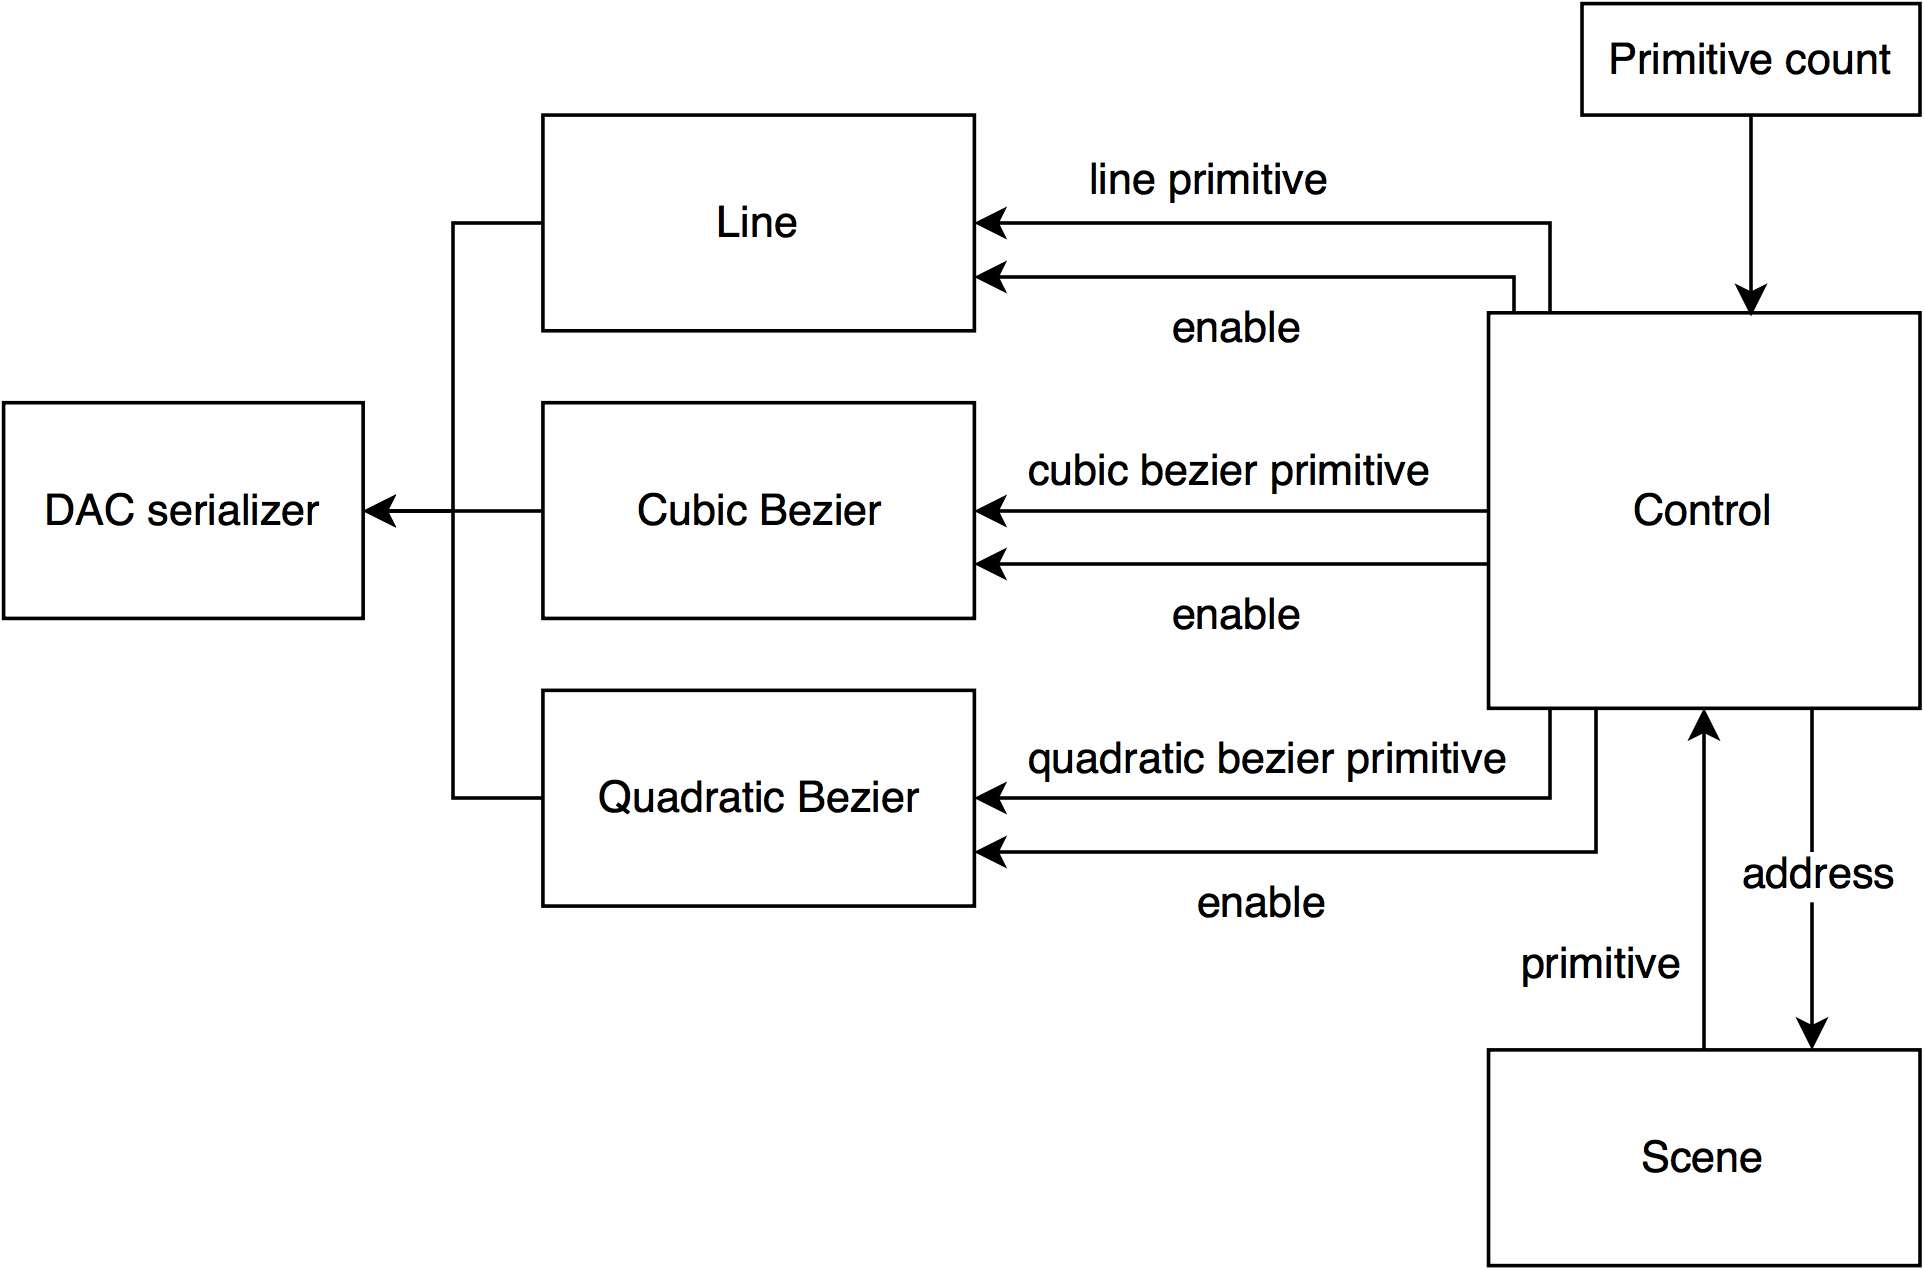
\includegraphics[width=\linewidth]{images/dac-output.png}
    \caption{RTL sketch of the \vthreek DAC output module.}
    \label{fig:dac-output}
\end{figure}

The primary output of the processor is the vector output.
This output is driven by two DACs that converts digital data from the FPGA to voltages that represents x and y coordinates.
The DACs used are 16-bit which gives us and effective resolution of 65536 by 65536 without taking into account the noise on the output voltage.
These DACs have a serial interface and needs 3 signals each to operate; data, clock, and a sync signal. 
In order to set an output value on a DAC the sync signal needs to be pulled from high to low then it needs 8 control bits followed by 16 data bits. 
After this, the sync signal need to be pulled high again in order to set the output value. 
The sync signal can be pulled high before this in order to abort the operation.
Clock and sync signal are shared between the DACs in this system in order to make them change their output synchronously.

The maximum clock frequency of the DACs is 30MHz. 
Since it needs to clock on 24 values per output change as well as the sync signal toggle the effective output maximum will be 30MHz/25=1.2MHz.
However in the implementation the DACs were unstable if clocked any faster than 20MHz which limits the output rate to around 800KHz.

\begin{cequation}[H]
	\begin{equation*}
		\mathbf{B}(t)=\mathbf{P}_0 + t(\mathbf{P}_1-\mathbf{P}_0)=(1-t)\mathbf{P}_0 + t\mathbf{P}_1 \mbox{ , } 0 \le t \le 1
	\end{equation*}
	\caption{Linear Bezier curve}
\end{cequation}

\begin{cequation}[H]
	\begin{equation*}
		\mathbf{B}(t) = (1 - t)^{2}\mathbf{P}_0 + 2(1 - t)t\mathbf{P}_1 + t^{2}\mathbf{P}_2 \mbox{ , } 0 \le t \le 1
	\end{equation*}
	\caption{Quadratic Bezier curve}
\end{cequation}

\begin{cequation}[H]
	\begin{equation*}
		\mathbf{B}(t)=(1-t)^3\mathbf{P}_0+3(1-t)^2t\mathbf{P}_1+3(1-t)t^2\mathbf{P}_2+t^3\mathbf{P}_3 \mbox{ , } 0 \le t \le 1
	\end{equation*}
	\caption{Cubic Bezier curve}
\end{cequation}


\section{Raster output}

This output uses HDMI to output a rasterized image of the internal vector representation.
In order to drive this output each primitive in the scene memory needs to be rasterized into a frame-buffer that is in turn TMDS encoded before it is sent over HDMI to a display.